\documentclass{article}
\usepackage[english]{babel}
\usepackage[utf8]{inputenc}
\usepackage[T1]{fontenc}
\usepackage{graphicx}
\usepackage[colorinlistoftodos]{todonotes}
\usepackage[colorlinks=true, allcolors=tudelftblue]{hyperref} %sets hyperlink colour
\usepackage{caption}
\usepackage{subcaption}
\usepackage{xcolor}
\usepackage{roboto} % for Roboto Slab font
\usepackage{float}
\usepackage{titling} 
\usepackage{blindtext}\usepackage{titlesec}
\usepackage[square,sort,comma,numbers]{natbib}
\usepackage[colorinlistoftodos]{todonotes}
\usepackage{tikz}
\usepackage{geometry}
\usepackage{sectsty}
\usepackage{amsmath}
\usepackage{tikzpagenodes}
\usepackage{booktabs}
\usepackage{longtable}
\usepackage{titlesec}
\usepackage{listings}
\definecolor{tudelftdarkblue}{RGB}{0,0,0}
\definecolor{tudelftcyan}{RGB}{209,65,36}
\definecolor{tudelftblue}{RGB}{99, 102, 106}
\geometry{a4paper, margin=2cm}
\allsectionsfont{\color{black}} %sets colour for all headers
\usepackage{helvet}
\renewcommand{\familydefault}{\sfdefault}
\sectionfont{\fontfamily{RobotoSlab-TLF}\selectfont}
%%%%%%%%%%%%%%%%%%%%%%%%%%%%%%%%%%%%%%%%%%%%%%%%%%%%%%%%%
\begin{document}

\begin{titlepage}
    \fontfamily{RobotoSlab-TLF}\selectfont 

    \begin{center}
%%%%%%%%%%%%%%%%%%%%%%%%%%%%%%%%%%%%%%%%%%%%%%%%%%%%%%%%%%UNCOMMENT THE FOLLOWING FOR LESS "PLAIN" TITLE PAGE (SELECT WITH MOUSE AND PRESS CTRL AND /)

    % \begin{tikzpicture}[remember picture,overlay]
    %     % Set seed for random number generator
    %     \pgfmathsetseed{4}
    %     % Define the text area to avoid
    %     \path (current page text area.south west) rectangle (current page text area.north east);
    %     % Adding circles spread over the entire page
    %     \foreach \x in {1,...,1000}
    %         \draw[tudelftdarkblue] (current page.south west) ++(rand*\paperwidth,rand*\paperheight) circle (rand*0.3);
    %     % Define coordinates for the corners of the white box
    %     \coordinate (A) at ([shift={(-8cm,12cm)}]current page.center);
    %     \coordinate (B) at ([shift={(8cm,-5cm)}]current page.center);
    %     % Draw the white background box
    %     \fill[white] (A) rectangle (B);
    %     % Adding equations as background features
    %     \node[anchor=center,rotate=20,text=tudelftcyan] at ([shift={(-7cm,-2cm)}]current page.center) {\fontsize{18}{22}\selectfont
    %     $\nabla^2 T - \frac{1}{\alpha}\frac{\partial T}{\partial t} = 0$};
    %     \node[anchor=center,rotate=-15,text=tudelftcyan] at ([shift={(5cm,-4cm)}]current page.center) {\fontsize{18}{22}\selectfont
    %     $\frac{\partial \rho}{\partial t} + \nabla \cdot (\rho \mathbf{v}) = 0$};
    %     \node[anchor=center,rotate=20,text=tudelftcyan] at ([shift={(6cm,4cm)}]current page.center) {\fontsize{18}{22}\selectfont
    %     $a^2 + b^2 = c^2$};
    %     \node[anchor=center,rotate=10,text=tudelftcyan] at ([shift={(7cm,-2cm)}]current page.center) {\fontsize{18}{22}\selectfont
    %     $E = \frac{\sigma}{\varepsilon}$};
    %     \node[anchor=center,rotate=-10,text=tudelftcyan] at ([shift={(-6cm,4cm)}]current page.center) {\fontsize{18}{22}\selectfont
    %     $F = ma$};
    %     \node[anchor=center,rotate=5,text=tudelftcyan] at ([shift={(-4cm,-5cm)}]current page.center) {\fontsize{18}{22}\selectfont
    %     $Q = -\frac{kA}{\mu} \frac{\Delta P}{L}$};
    % \end{tikzpicture}
%%%%%%%%%%%%%%%%%%%%%%%%%%%%%%%%%%%%%%%%%%%%%%%%%%%%%%%%%%
    \vspace*{2cm}  % Spazio iniziale per separare la parte superiore della pagina
    
    % Immagine centrata
    
\includegraphics[width=0.6\textwidth]{images/Logo_C_Positivo_Colore.png}

    \vspace*{2cm}  % Spazio tra immagine e il testo sottostante

    {\Huge \textbf{\textcolor{black}{Tesina per il corso di Basi di Dati \\ a.a 2024-2025 }}}\\[1.5cm]
    {\Huge \textbf{\textcolor{black}{InnovaCity}}}\\[0.5cm]
    {\Large \textbf{\textcolor{tudelftdarkblue}{Studenti:}}}\\[0.5cm]
    \begin{tabular}{c}
        \Large \textcolor{tudelftdarkblue}{Canovi Stefano (176711)} \\ 
        \Large \textcolor{tudelftdarkblue}{Frattolillo Mattia (177214)} \\ 
    \end{tabular}\\[2cm]
    
    \vspace*{1cm}
    {\Large \textbf{\textcolor{tudelftdarkblue}{Progetto di una base di dati\\ per la gestione di una città sostenibile }}}\\[1.3cm]
    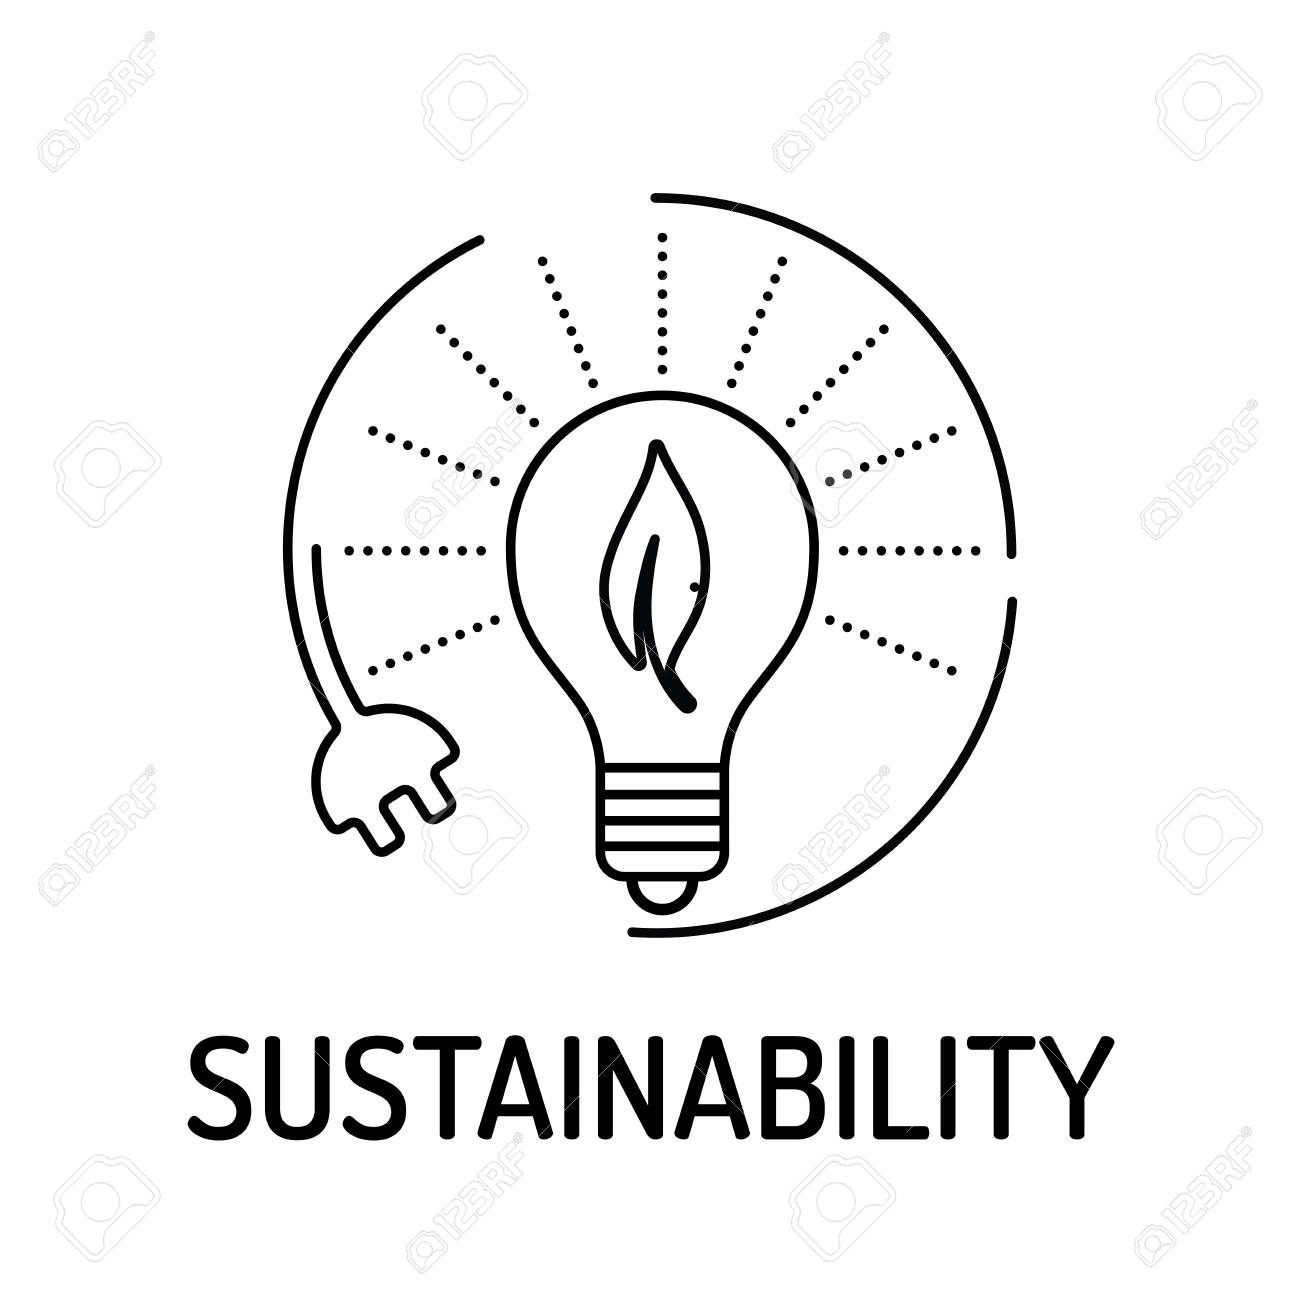
\includegraphics[width=0.3\textwidth]{images/SOSTENIBILITA.png}

    \end{center}  % Fine del centering
\end{titlepage}

%%% Create a table of contents
\tableofcontents
\newpage

%---------------------PAGINA DI DESCRIZIONE DEL DB E ANALISI PRIMA CLASSE DI UTENTE-------------------

\section*{1.Analisi dei requisiti e progetto delle viste}
\addcontentsline{toc}{section}{1.Analisi dei requisiti e progetto delle viste}
\raggedright

\vspace{-0.5cm}
\noindent\rule{\textwidth}{1pt}
\vspace{0.5cm}

\textbf{Titolo della tesina:} \textit{Progetto di una base di dati per un'area urbana sostenibile}

\par\vspace{0.5cm}

Il presente elaborato descrive la progettazione di un sistema informativo orientato alla gestione e al monitoraggio delle iniziative legate alla sostenibilità urbana in una città moderna e attenta allo sviluppo green.

\par\vspace{0.3cm}

Il database è concepito per raccogliere, strutturare e analizzare dati su questo tipo di città, con l'obiettivo di offrire un supporto concreto nella pianificazione strategica e operativa delle attività urbane, e costituire un modello replicabile per altre realtà urbane interessate a intraprendere un percorso verso la sostenibilità.

\par\vspace{0.3cm}

Attraverso un'architettura flessibile e relazionale, la base di dati permette il monitoraggio continuo di vari ambiti come il coinvolgimento dei cittadini nello sviluppo di infrastrutture e prodotti green, le collaborazioni e partnership tra aziende (più o meno etiche) per offrire prodotti sostenibili e di qualità alla società, e l'utilizzo efficiente delle risorse naturali.

\par\vspace{0.3cm}

Il sistema coinvolge molteplici attori, sia pubblici che privati, i quali interagiscono all’interno di un ecosistema urbano integrato, ciascuno contribuendo con dati e funzioni specifiche. Tra questi si possono individuare tre principali classi di utenti:

\begin{itemize}
    \item \textbf{Cittadini}
    \item \textbf{Aziende private}
    \item \textbf{Enti pubblici}
\end{itemize}

\titleformat{\subsection}[block]
  {\normalfont\bfseries\Large}
  {}
  {0pt}
  {}

\vspace{0.3cm}
\subsection*{1.1Formulazione e analisi dei requisiti per i Cittadini}
\vspace{0.6cm}

I \textbf{cittadini}, identificati tramite \textit{codice fiscale}, \textit{nome}, \textit{cognome} e \textit{residenza}, rappresentano una componente fondamentale all'interno di questa realtà urbana sostenibile.

\par\vspace{0.3cm}

Essi hanno la possibilità di contribuire attivamente alla crescita della città attraverso la pubblicazione delle proprie idee all'interno di un apposito albo cittadino digitale, distinguendosi così dagli altri utenti come ideatori di potenziali prodotti o servizi orientati alla sostenibilità.

\par\vspace{0.3cm}

Ogni idea proposta è associata a un titolo, una descrizione e una data di inserimento, e può riguardare vari ambiti.

\par\vspace{0.3cm}

Oltre alla proposta di idee, i cittadini possono rilasciare feedback, uno strumento essenziale per valutare il grado di apprezzamento da parte della comunità e per misurare l'effettivo impatto e progresso delle iniziative, sia in termini di affluenza che di sostenibilità.

\par\vspace{0.3cm}

I feedback possono essere espressi sia sull'idea iniziale che sul prodotto finale, ovvero sul risultato concreto del processo di definizione, applicazione e realizzazione del progetto basato sull'idea stessa.

\par\vspace{0.3cm}

Questa doppia valutazione risulta utile per analizzare la coerenza tra l'idea e la sua effettiva attuazione, e per comprendere se il prodotto ha mantenuto o superato le aspettative iniziali.

\par\vspace{0.3cm}

I nuovi prodotti sostenibili vengono infine presentati alla comunità attraverso eventi pubblici, manifestazioni organizzate con l'obiettivo di offrire una prima esposizione delle soluzioni sviluppate.

\par\vspace{0.3cm}

Gli eventi sono strutturati in settori tematici, permettendo a ogni cittadino di orientarsi facilmente verso le aree di proprio interesse.

%-------------------------------------------------------------------------------------------------------

\newpage
\titleformat{\subsection}[block]
  {\normalfont\bfseries\Large}
  {}
  {0pt}
  {}

\vspace{-1.3cm}
\subsection*{Glossario dei concetti per i cittadini}
\vspace{0.6cm}

\begin{longtable}{|p{3cm}|p{6.5cm}|p{2.5cm}|p{3cm}|}
\hline
\textbf{Termine} & \textbf{Descrizione} & \textbf{Sinonimi} & \textbf{Collegamenti} \\
\hline
\endfirsthead
\hline
\textbf{Termine} & \textbf{Descrizione} & \textbf{Sinonimi} & \textbf{Collegamenti} \\
\hline
\endhead

Cittadino & Utente identificato da codice fiscale, nome, cognome e residenza, che può proporre idee e lasciare feedback. & Utente & Idea, Feedback, Evento \\
\hline

Idea & Proposta inserita da un cittadino, associata a titolo, descrizione e data. Può riguardare vari ambiti sostenibili. & Proposta, Iniziativa & Cittadino, Feedback, Progetto \\
\hline

Feedback & Valutazione lasciata da un cittadino su un'idea o su un prodotto finale, utile per misurare apprezzamento e impatto. & Opinione, Commento & Cittadino, Idea, Prodotto \\
\hline

Prodotto & Risultato concreto derivante da un progetto di un' idea. Oggetto della valutazione finale tramite feedback. & Prodotto finale, Soluzione & Progetto, Feedback, Evento \\
\hline

Evento & Manifestazione pubblica dove vengono presentati i prodotti sostenibili alla comunità. & Presentazione, Manifestazione & Cittadino, Prodotto, Settore Tematico \\
\hline

Settore Tematico & Area tematica in cui sono suddivisi gli eventi, per facilitare la fruizione da parte dei cittadini. & Tema, Categoria & Evento, Idea\\
\hline

Albo cittadino digitale & Spazio online in cui i cittadini possono pubblicare idee sostenibili. & Bacheca digitale & Cittadino, Idea \\
\hline

\end{longtable}

\titleformat{\subsection}[block]
  {\normalfont\bfseries\Large}
  {}
  {0pt}
  {}

\vspace{0.3cm}
\subsection*{Schema scheletro per i Cittadini}
\vspace{0.6cm}

\begin{figure}[H]
    \centering
    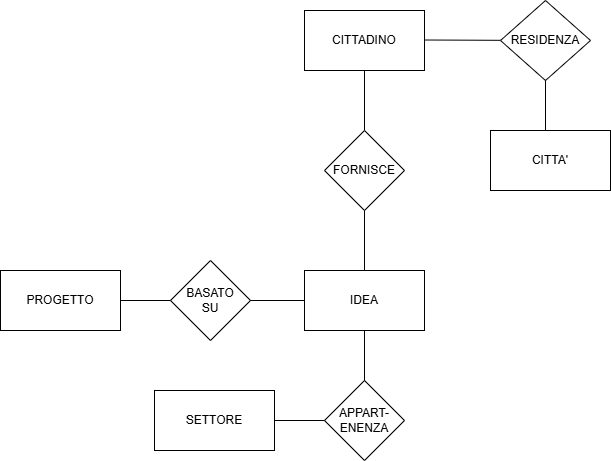
\includegraphics[width=0.8\textwidth]{images/SCHELETRO_CITTADINO.drawio.png}
    \caption{Schema del modello di sostenibilità urbana}
    \label{fig:schema-sostenibilita}
\end{figure}

\end{document}


%All other official TU Delft colours
\definecolor{donkerblauw}{RGB}{12, 35, 64}
\definecolor{turkoois}{RGB}{0, 184, 200}
\definecolor{blauw}{RGB}{0, 118, 194}
\definecolor{paars}{RGB}{111, 29, 119}
\definecolor{roze}{RGB}{239, 96, 163}
\definecolor{framboos}{RGB}{165, 0, 52}
\definecolor{rood}{RGB}{224, 60, 49}
\definecolor{oranje}{RGB}{237, 104, 66}
\definecolor{geel}{RGB}{255, 184, 28}
\definecolor{lichtgroen}{RGB}{108, 194, 74}
\definecolor{donkergroen}{RGB}{0, 155, 119}
%You can use these to change the hyperlink colour or the colour of the header or whatever. Glück Auf!